\section{Результаты}
To prove the feasibility of the proposed approach, link-layer simulations
(LLS) were performed, comparing the proposed scheme with the cases of ideal
PA and no-compensation case for a given PA model. The model based
parameters of the typical real power amplifiers in the 30-70 GHz band [15]
was used along with newly developed model for the 100-200 GHz. Basic LLS
simulation assumptions are summarized in Table 1.

\begin{figure}[h!]
    \centering
    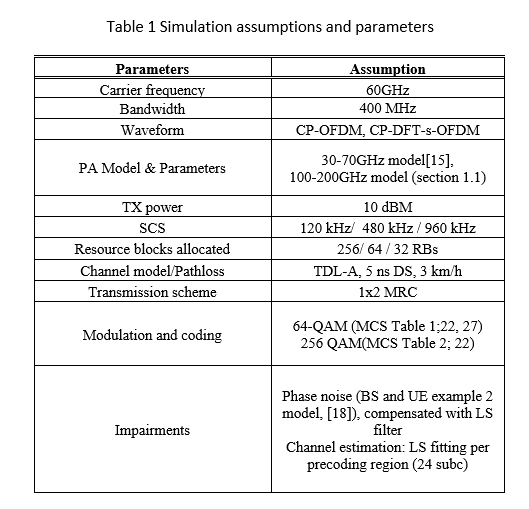
\includegraphics[width=0.5\linewidth]{figs/parameters table.png}
\end{figure}

\subsection{Результаты симуляций для модели 30-70 ГГц}

\begin{figure}[h!]
    \centering
    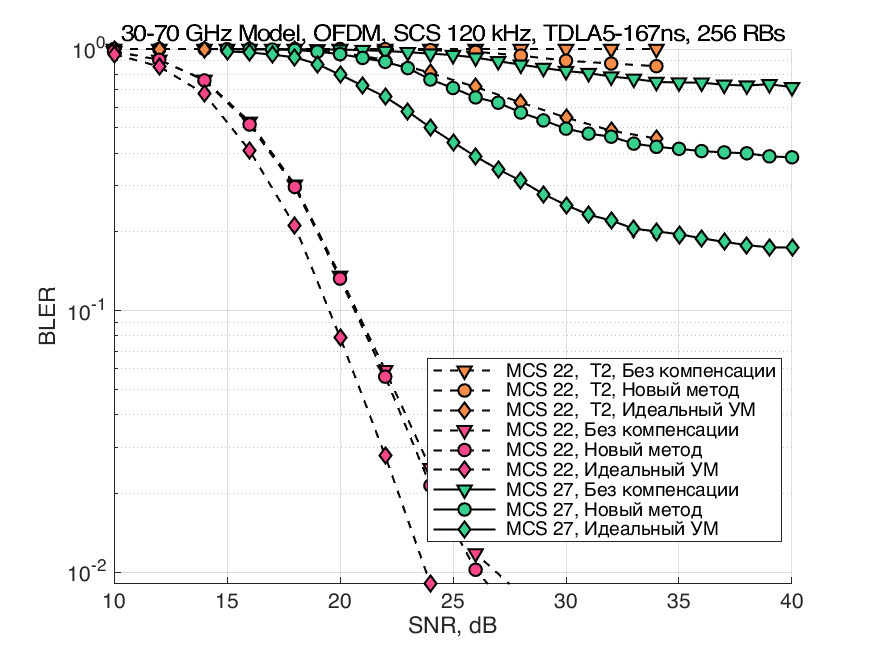
\includegraphics[width=0.49\linewidth]{figs/res/ofdm/OFDM_Nokia_SCS120_MCS22_27.png}
    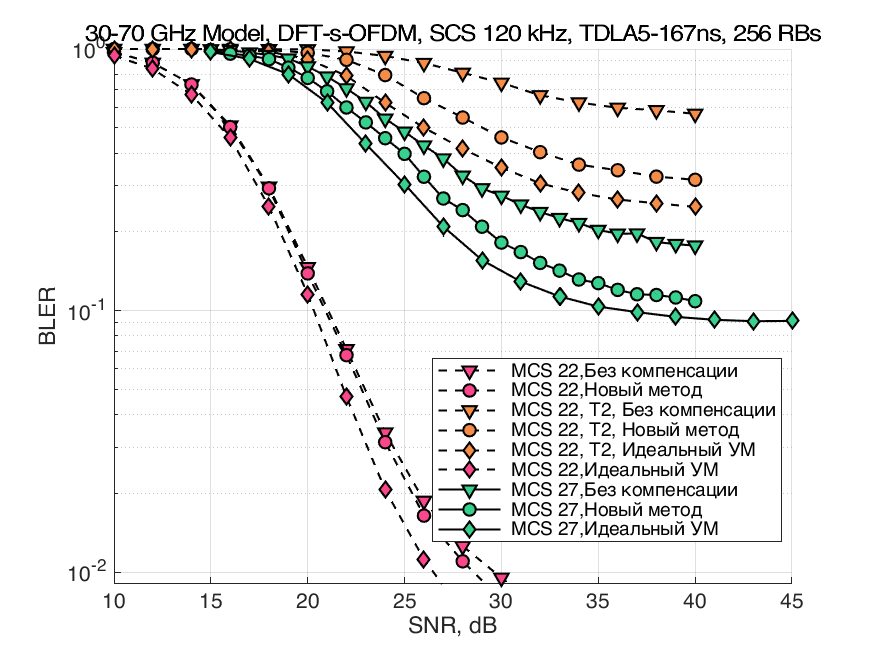
\includegraphics[width=0.49\linewidth]{figs/res/dftsofdm/DFT-s-OFDM_Nokia_SCS120_MCS22_27.png}
    \caption{BLER for SCS 120 kHz, 64-QAM/256 QAM for OFDM (left) and DFT-s-OFDM(right)}
    \label{fig:res3070_scs120}
\end{figure}

\begin{figure}[h!]
    \centering
    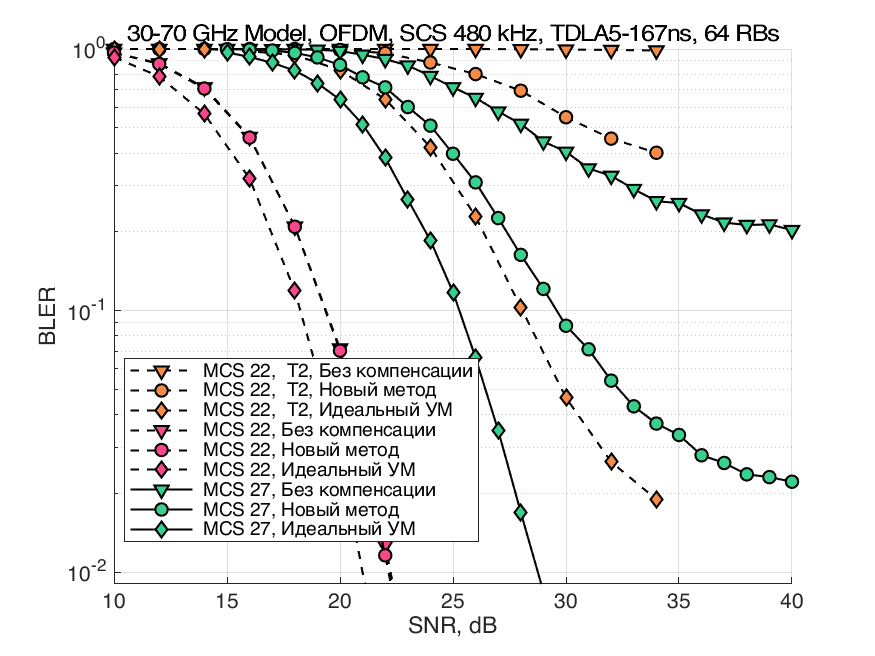
\includegraphics[width=0.49\linewidth]{figs/res/ofdm/OFDM_Nokia_SCS480_MCS22_27.png}
    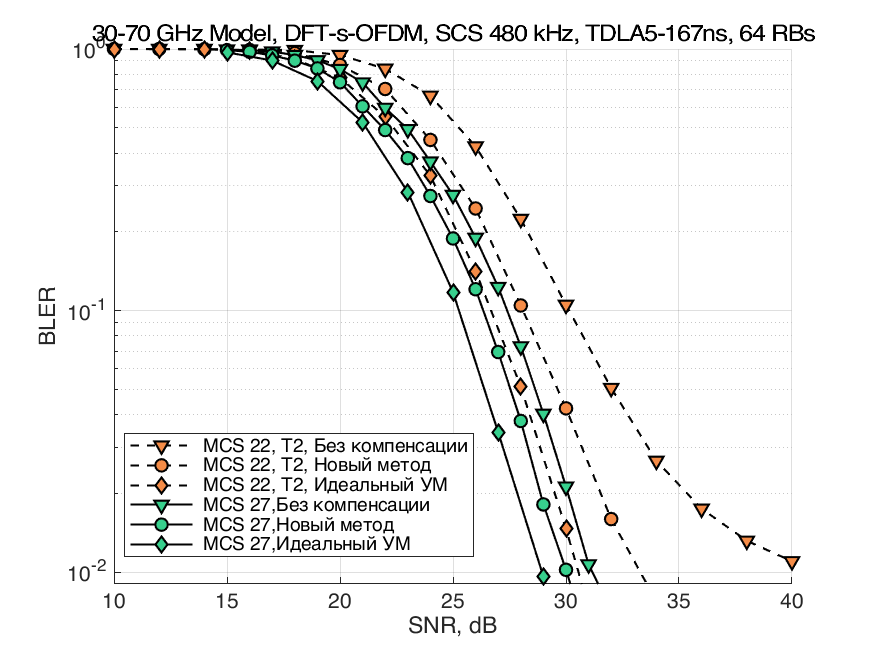
\includegraphics[width=0.49\linewidth]{figs/res/dftsofdm/DFT-s-OFDM_Nokia_SCS480_MCS22_27.png}
    \caption{SCS480}
    \label{fig:res3070_scs480}
\end{figure}

\begin{figure}[h!]
    \centering
    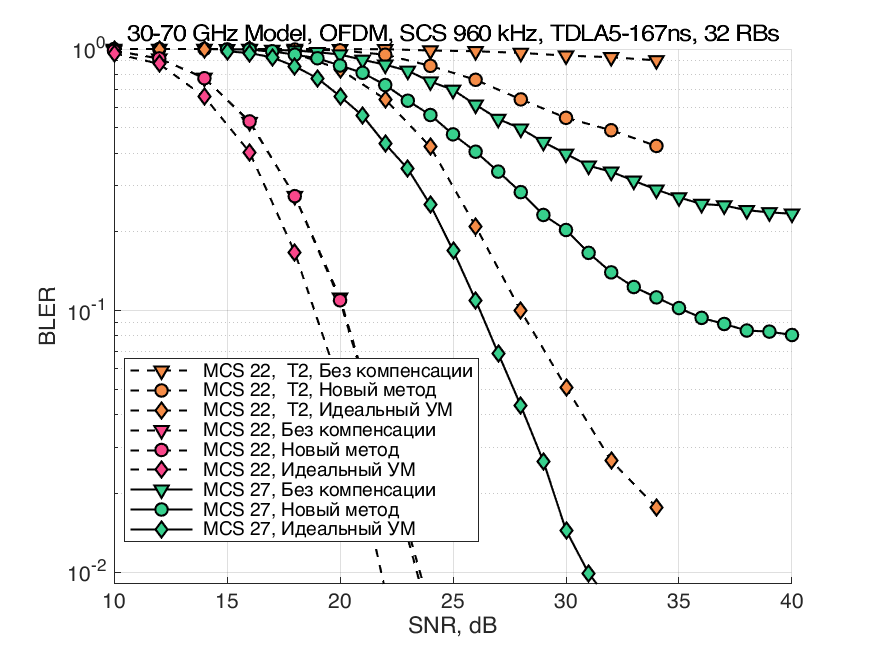
\includegraphics[width=0.49\linewidth]{figs/res/ofdm/OFDM_Nokia_SCS960_MCS22_27.png}
    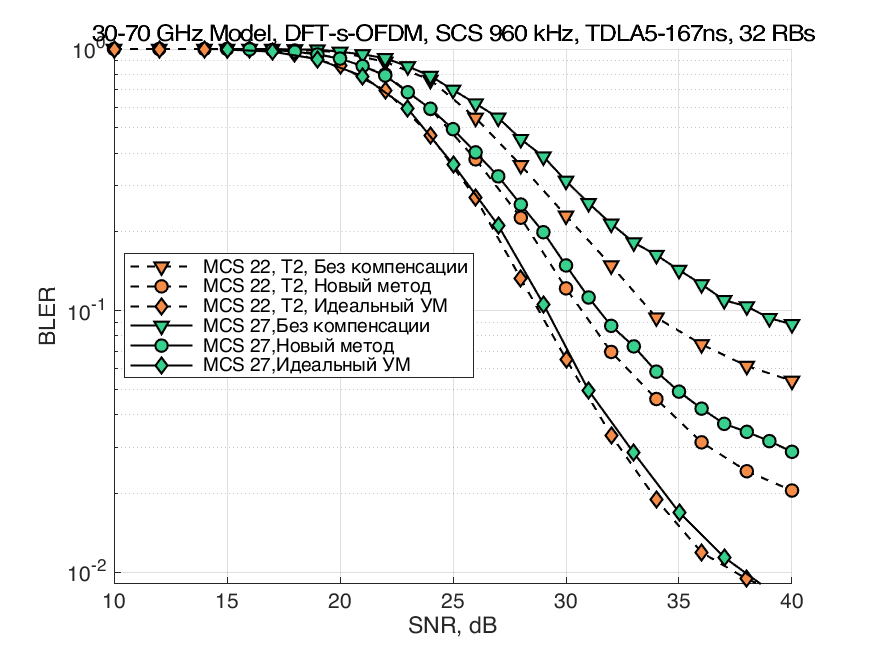
\includegraphics[width=0.49\linewidth]{figs/res/dftsofdm/DFT-s-OFDM_Nokia_SCS960_MCS22_27.png}
    \caption{SCS960}
    \label{fig:res3070_scs960}
\end{figure}

\subsection{Результаты симуляций для модели 100-200 ГГц}

\begin{figure}[h!]
    \centering
    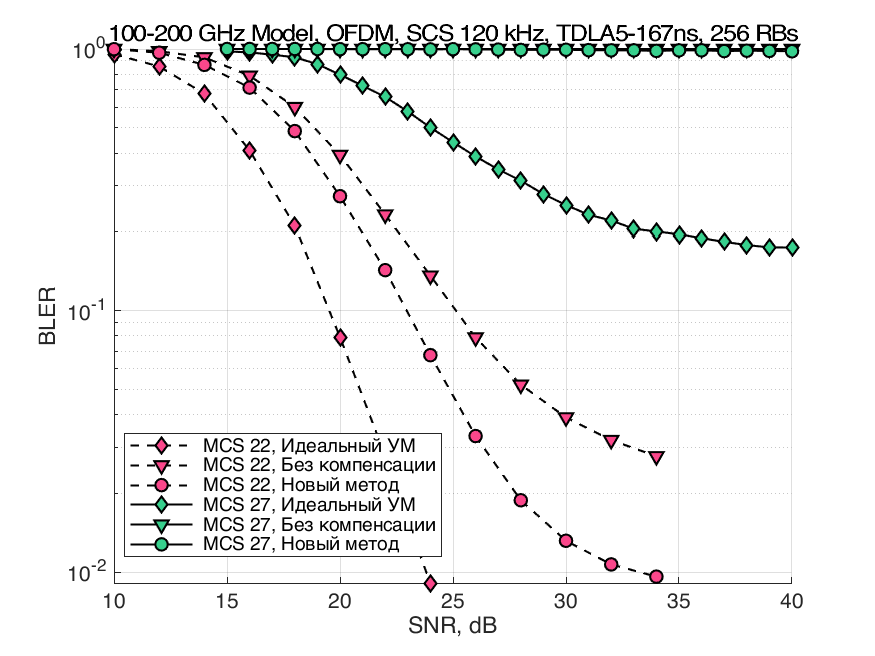
\includegraphics[width=0.49\linewidth]{figs/res/ofdm/OFDM_SubTHz_SCS120_MCS22_27.png}
    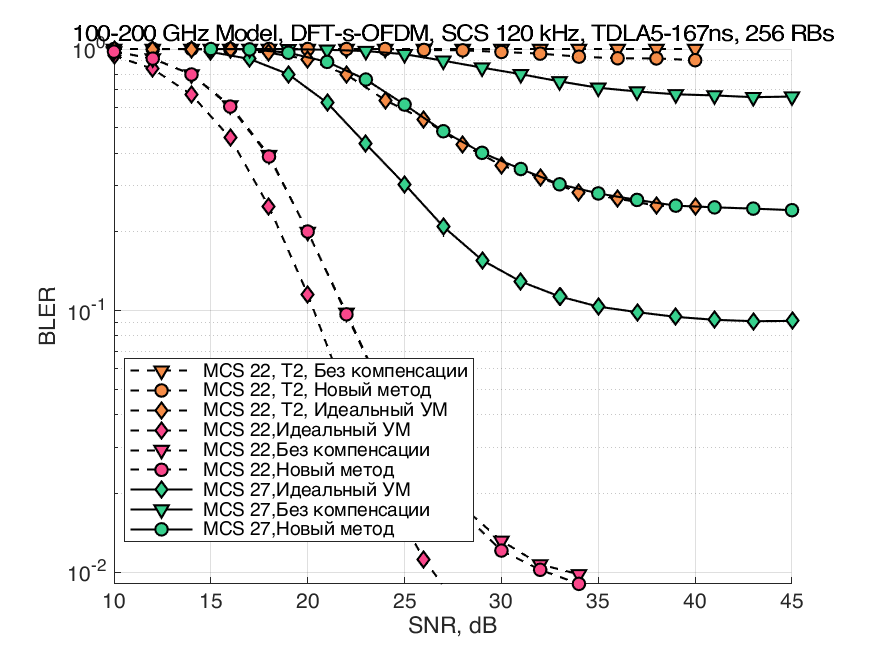
\includegraphics[width=0.49\linewidth]{figs/res/dftsofdm/DFT-s-OFDM_SubTHz_SCS120_MCS22_27.png}
    \caption{SCS120}
    \label{fig:res100200_scs120}
\end{figure}

\begin{figure}[h!]
    \centering
    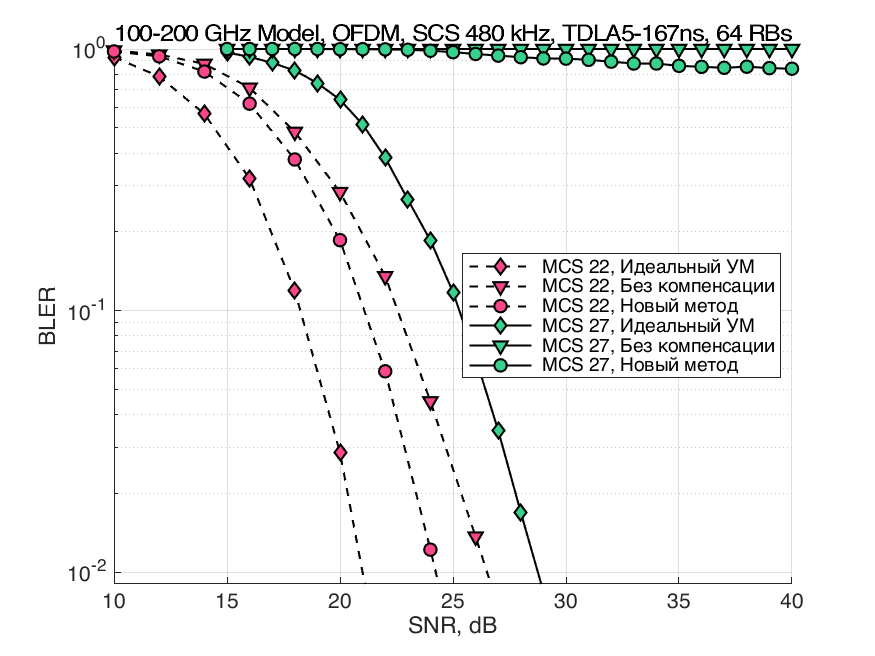
\includegraphics[width=0.49\linewidth]{figs/res/ofdm/OFDM_SubTHz_SCS480_MCS22_27.png}
    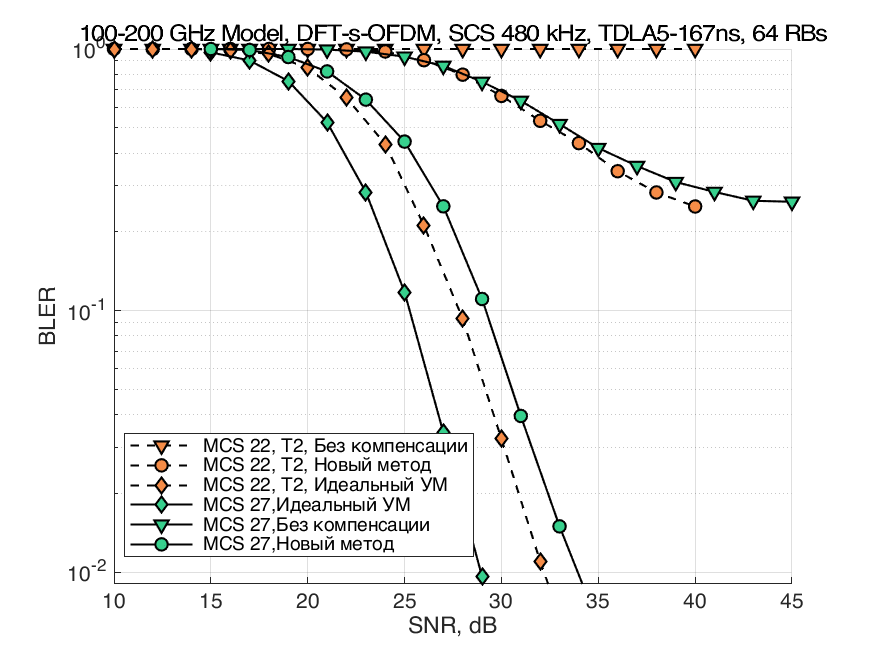
\includegraphics[width=0.49\linewidth]{figs/res/dftsofdm/DFT-s-OFDM_SubTHz_SCS480_MCS22_27.png}
    \caption{SCS480}
    \label{fig:res100200_scs480}
\end{figure}

\begin{figure}[h!]
    \centering
    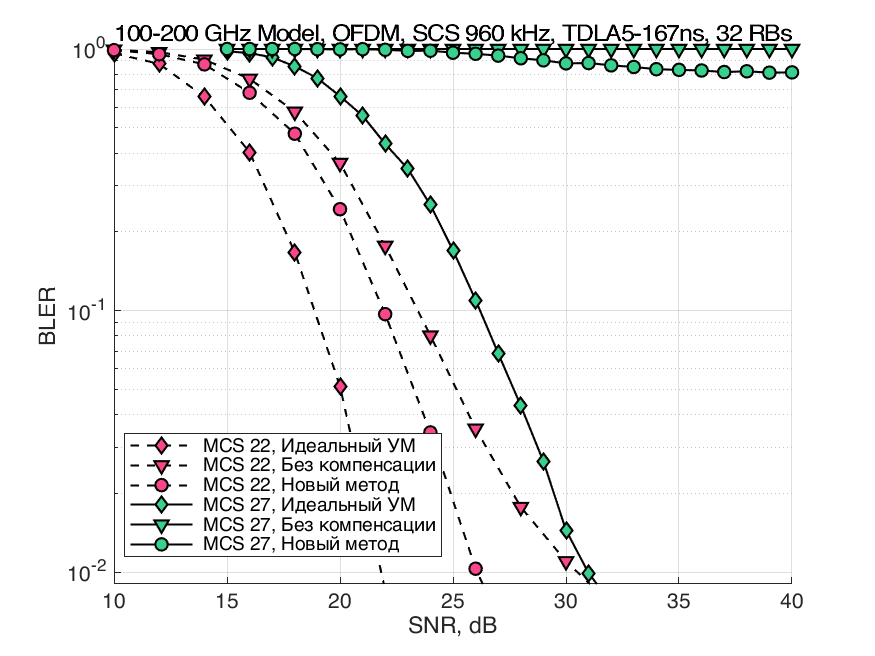
\includegraphics[width=0.49\linewidth]{figs/res/ofdm/OFDM_SubTHz_SCS960_MCS22_27.png}
    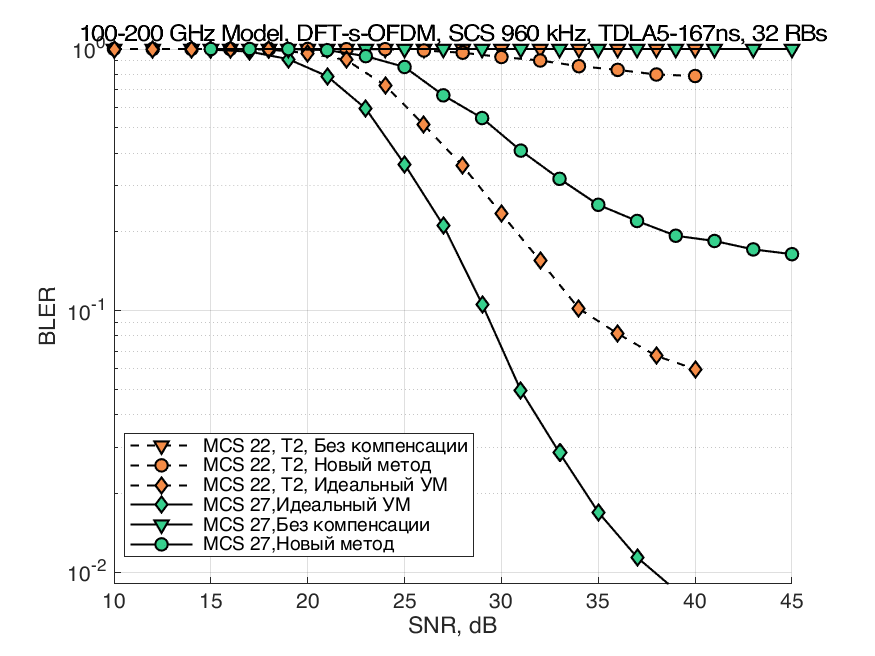
\includegraphics[width=0.49\linewidth]{figs/res/dftsofdm/DFT-s-OFDM_SubTHz_SCS960_MCS22_27.png}
    \caption{SCS960}
    \label{fig:res100200_scs960}
\end{figure}


% \subsection{Последовательность применения компенсаций} Предложенный метод
% предполагается использовать до компенсации фазового шума (PN), однако
% другие последовательности были рассмотрены и рассчитаны. Применение
% компенсации нелинейности УМ после компенсации PN показало определенное
% ухудшение производительности, поэтому компенсация нелинейности УМ везде
% производилась до компенсации фазовых шумов в большинстве расчетов.
% Примеры результатов, в которых сравнивается разный порядок компенсации
% фазовых шумов и нелинейности усилителя приведены на Figure 10.

% \subsection{Наблюдения}

% • Для модели УМ в диапазоне 30-70 ГГц (подходящего для диапазона АК2 и
% выше) улучшение наблюдается только для модуляций высокого порядка o Для
% SCS 120 кГц, отрицательные эффекты фазового шума значительны, и при таких
% искажениях результаты компенсации нелинейности УМ незначительны o Для SCS
% 480 и 960 кГц, в которых возможна более эффективная компенсация фазового
% шума, в определенный момент влияние нелинейности УМ становится основным
% ограничивающим фактором. В этом случае компенсация нелинейности УМ может
% улучшить результат на несколько дБ или совсем избавиться от искажений,
% внесенных УМ. • Для модели 100-200 ГГц, влияние нелинейности УМ
% увеличивается, и в большинстве случаев превосходит влияние фазовых шумов
% o Предложенный метод компенсации демонстрирует улучшение результата для
% MCS 22 и выше • Не смотря на возможность различных имплементаций,
% диктуемая логикой последовательность компенсации искажений в порядке,
% обратному их появлению в системе оказывается оптимальным. Таким образом,
% искажения должны быть компенсированы в порядке канал, усилитель мощности,
% фазовые шумы.  